\documentclass[pdftex,12pt,a4paper]{article} 
% margin size
\usepackage[margin=1in]{geometry}

% Math and algorithms
\usepackage{amsmath,amssymb,amsthm,esint}  % For both in-line and equation mode
\usepackage{bbm}
\usepackage{mathdots}
\usepackage{bm}
\usepackage{algorithm}
\usepackage{algorithmic} % Algorithm styles, need to be nested for the example shown
\usepackage{aliascnt}
\numberwithin{equation}{section} % Numbering of our equations per section
\newtheorem{theorem}{Theorem}
\newtheorem{definition}{Definition}
\newtheorem{proposition}{Proposition}
\newtheorem{corollary}{Corollary}
\newtheorem{remark}{Remark}

\usepackage{setspace} %Spacing on the front page for crest and titles
\usepackage[]{fncychap} % Styles can be Sonny, Lenny, Glenn, Conny, Rejne, Bjarne and Bjornstrup
\usepackage[hyphens]{url} % Deals with hyphens in urls to make them clickable
\usepackage{xcolor} % Great if you want coloured text

% Figures
\usepackage{wrapfig}
\usepackage{graphicx} % Inserting images
\graphicspath{ {../figures/} } 
\usepackage{caption}
\usepackage{float}

% Tables
\usepackage{tabularx}
\usepackage{multirow} 
\renewcommand{\arraystretch}{1.5}

% Appendix
\usepackage{appendix} 

\usepackage{natbib}
\usepackage{comment}

% Tikz figures
\usepackage{tikz}
\newcommand{\ImageWidth}{14cm} 
\usetikzlibrary{decorations.pathreplacing,positioning, arrows.meta} 

% Fancy headers and footnotes
\usepackage{fancyhdr}
\usepackage[symbol]{footmisc}
\renewcommand{\thefootnote}{\fnsymbol{footnote}} 

% Hyperlinks and auto-references
\usepackage[hidelinks]{hyperref}  
\def\sectionautorefname{Section}
\def\appendixname{Appendix}
\newcommand{\propositionautorefname}{Proposition}
\newcommand{\definitionautorefname}{Definition}
\newcommand{\corollaryautorefname}{Corollary}  

\setlength{\footnotesep}{0.5cm}
%%%%%%%%%%%%%%%%%%%%%%%%%% DOCUMENT STARTS %%%%%%%%%%%%%%%%%%%%%%%%%%%%% 

\begin{document} 
% Front page 
\pagestyle{empty}
% Dissertation Title
\begin{center}
	\textbf{\begin{huge}
		How Does Varying the Length of Prime Factors in RSA Key Generation Impact the Complexity of the Encrypted Output?\\ 
	\end{huge}} 
	\vspace{10mm}
\end{center}

% Supervisor, Department and Date
\begin{center}
	\textbf{\large Santiago Hernández\\} 
	\vspace{5mm}
	\textbf{\large International Baccalaureate program}\\ 
    %\vspace{2mm}
    {\large Mathematics\\} 
	%{\large January 2023\\}
	\vspace{5mm}
\end{center} 

% \begin{center}
% 	\textbf{\large Candidate Code: }\large kxm245 \\
% \end{center}

% Abstract
\begin{center}

\end{center} 
\vspace{0mm}

% Word count
\begin{center}
    \vspace{10mm}
	\vspace{2mm}
    \textbf{Page Count:} 12\\
\end{center}
%\vspace{10mm}  
%\renewcommand{\headrulewidth}{0pt} 
\tableofcontents
\clearpage
\renewcommand{\thefootnote}{\arabic{footnote}}
\pagestyle{fancy}
\fancyhf{}
\setlength{\headheight}{14.49998pt}
\addtolength{\topmargin}{-2.49998pt} 
\lhead{RSA Complexity}
\def\layersep{2.5cm}
\pagenumbering{arabic}
\lfoot{\centering \thepage}
\onehalfspacing 

% Sections
\section{Introduction}
\label{sec:section1}
In a society where technology is used daily to transmit sensitive information worldwide, data encryption has become increasingly important since it ensures that data transmitted over the internet remains private and secure. Due to this, many cryptographic systems have been implemented to encrypt data over the internet, with one of the oldest and most widely used encryption methods being RSA encryption.

RSA encryption is an algorithm presented in 1977 by Ron Rivest, Adi Shamir, and Leonard Adleman \citep{Rivest_Shamir_Adleman_1977}. RSA’s security relies on the difficulty of factoring the product of two large prime numbers and is an algorithm that implements many mathematical concepts.

This paper mainly falls under two branches of mathematics: number theory, which deals with the study of integers and their properties, and algebraic structures, which involves the study of sets, particularly in the context of integers modulo $n$ ($\mathbb{Z}_n$), where $n$ is a product of two large prime numbers. This paper intends to explore the algorithm behind RSA, along with its mathematical properties, to assess RSA’s security. This paper is structured as follows: In \autoref{sec:section2}, I introduce the underlying mathematics behind the RSA algorithm. In \autoref{sec:section3}, I present the RSA algorithm and explain how and why it works. \autoref{sec:section4} explores a different method for deriving RSA private exponents. \autoref{sec:section5} contains a detailed example of the key generation, encryption, and decryption processes; while in \autoref{sec:section6}, I explain the framework used to assess the security of RSA. Lastly, \autoref{sec:section7} presents concluding remarks and assesses the security of RSA encryption based on the framework presented in \autoref{sec:section6}.





\section{Underlying Mathematics}\label{sec:section2}
RSA relies on certain mathematical principles that make it work; one of these concepts is the use of prime numbers. RSA encryption uses large primes that are multiplied together to obtain a product. The security of RSA then rests on the fact that it is extremely difficult to factorize this product back into its original prime factors, especially if these are very large. 

Other mathematical concepts in RSA include modular arithmetic, which is used in the encryption and decryption process to perform operations on large primes efficiently, as well as coprime numbers. Because of the underlying mathematics, certain concepts are key to the inner workings of RSA; the mathematical concepts that form the basis of RSA encryption include Fermat's Little Theorem, Euler's Totient Function, and the Carmichael function. 

\subsection{Modular Arithmetic}\label{sec:section2.1}

In mathematics, modular arithmetic is a system of arithmetic for integers where numbers loop when reaching a certain value known as the modulus. An example of modular arithmetic is the 12-hour clock, which divides the day into two 12-hour periods. In 12-hour clocks, if the time is 5:00 now, in 8 hours, the time will be 1:00. Normal addition would result in $5 + 8 = 13$, but 13:00 is expressed as 1:00 on the clock face because clocks “loop” every 12 hours. In this example, it can be said that 13 is congruent to 1 modulo 12, which is written as

$$
13 \equiv 1 \pmod{12}
$$

\subsubsection{Integers Modulo n}\label{sec:section2.1.1}

Integers modulo $n$, denoted $\mathbb{Z}_n$, represent the set of integers from $0$ to $n-1$, where two integers are considered equivalent (or congruent) if their difference is divisible by $n$. In other words, integers $a, b$ are equivalent modulo $n$ (written as $a \equiv b \pmod{n}$) if $a - b$ is a multiple of $n$. Integers modulo $n$ can be expressed using the following notation:

$$
\mathbb{Z}_n = \{ 0,1,2, \ldots, n-1 \}.
$$

For example, $\mathbb{Z}_4 = {0,1,2,3}$ represents the integers modulo 4. Furthermore, $\mathbb{Z}_4$ has the following equivalences:

\[
\begin{aligned}
&1 \equiv 1 \pmod{4} \\
&2 \equiv 2 \pmod{4} \\
&3 \equiv 3 \pmod{4} \\
&4 \equiv 0 \pmod{4}
\end{aligned}
\]

In the example above, $4 \equiv 0 \pmod{4}$ because $4-0 = 4$, which is divisible by $4$. This means that in $\mathbb{Z}_4$, 4 is equivalent to 0 since they differ by a multiple of 4. Similarly, in $\mathbb{Z}_4$, $5 \equiv 1 \pmod{4}, 6 \equiv 2 \pmod{4}$, and so on. Integers modulo $n$ play a key role in RSA key generation.



\subsection{Group Theory}\label{sec:section2.2}

In mathematics, a group is defined as a non-empty set $G$ with a binary operation (denoted "$\cdot$") that combines any two elements $a$ and $b$ of $G$ to form an element of $G$, denoted $a \cdot b$, such that the following three requirements, known as Group axioms, are satisfied. 

\begin{itemize}
    \item \textbf{Associativity} \\
    For all $a,b,c$ in $G$, one has $(a \cdot b) \cdot c = a \cdot (b \cdot c)$ For example, $(1 + 2) + 3 = 1 + (2 + 3)$.
  \end{itemize}

  \begin{itemize}
    \item \textbf{Identity Element} \\
    There exists an element $e$ in $G$ such that, for every $a$ in $G$, one has $e \cdot a = a$ and $a \cdot e = a$, for example, $0 + 1 = 1, 1+ 0 = 1$. (In this example 0 is the group’s identity element).
  \end{itemize}

  \begin{itemize}
    \item \textbf{Inverse Element} \\
    For each $a$ in $G$, there exists an element $b$ in $G$ such that $a \cdot b = e$ and $b \cdot a = e$, where $e$ is the identity element. For each $a$, the element $b$ is unique; this is called the inverse of $a$ and is denoted as $a^{-1}$.  For example, $3 + (-3) = 0, -3 + 3 = 0$, where $a = 3, b=-3, e= 0$
  \end{itemize}
  
  In the group examples above, I described the set of integers under addition, which is commonly denoted as $\mathbb{Z}^{+}$ and satisfies all three of the group axioms. Groups are relevant to RSA encryption, as they are a crucial concept responsible for the relationship between public and private keys and the impossibility of algorithmically deriving a private key from a public key.



  \subsubsection{Cyclic Subgroups}\label{sec:section2.2.1}

  For any element $g$ in any group $G$, one can form the subgroup that consists of all its integer powers, meaning that the subgroup generated by the element $g$ consists of all powers of $g$, where $k$ ranges over all integers, this can be expressed as:
  
  $$
  \langle g \rangle = \{ g^k \mid k \in \mathbb{Z} \}.
  $$
  
  This is known as a cyclic subgroup and is commonly denoted as $\mathbb{Z}_n$. For example, consider a group of integers modulo 4, under addition, denoted as $\mathbb{Z}^{+}_{4}$. This group has four elements: $\{ 0,1,2,3 \}$. If we take the element 1, the powers of 1 in $\mathbb{Z}^{+}_{4}$ are $\{ 1,2,3,0 \}$, where $1^0 = 1, 1^1 = 1, 1^2 = 2, 1^3 = 3, 1^4 = 0$. Since all elements of $\mathbb{Z}^{+}_{4}$ can be generated by powers of 1, we say that $\mathbb{Z}^{+}_{4}$ is a cyclic group generated by 1.
  
  In general, a group is cyclic if an element $g$ exists in the group such that every element of the group can be written as a power of $g$.
  

\subsubsection{Multiplicative Group of Integers Modulo n}\label{sec:section2.2.2}
  
The multiplicative group of integers modulo $n$, denoted $\mathbb{Z}^{*}_{n}$, consists of all integers $a$ that range from 1 to $n-1$ that are coprime to $n$. For example, if $n = 8$, the integers from 1 to 7 are 1,2,3,4,5,6, and 7. However, the numbers that are coprime to 8 in this range are 1,3,5, and 7. Therefore $\mathbb{Z}^{*}_{8} = \{ 1,3,5,7 \}$.
  
\subsubsection{Modular Multiplicative Inverse}\label{sec:section2.2.3}

The modular multiplicative inverse of an integer $a$ modulo $m$ is another integer $b$ such that the product of $a$ and $b$ is congruent to 1 modulo $m$. In other words, $b$ is the multiplicative inverse of $a$ if $a \times b \equiv 1 \pmod{m}$. A modular multiplicative inverse for an integer $a$ modulo $m$ only exists if $a$ and $m$ are coprime, since that would mean that $a$ and $m$ have no common factors other than 1. If $a$ and $m$ have a common factor that is greater than 1, there is no multiplicative inverse since any multiple of $a$ will also be a multiple of the common factor shared with $m$, meaning it cant be congruent to 1. For example, to find the multiplicative inverse of $3 \pmod{7}$, we need to find an integer $b$ such that $3 \times b \equiv 1 \pmod{7}$. If we then try out multiple values for $b$, we find that $3 \times 5 \equiv 15 \equiv 1 \pmod{7}$. Therefore, the modular multiplicative inverse of $3 \pmod{7}$ is 5. The modular multiplicative inverse is a crucial concept in RSA as it ensures that a private key can be used to decrypt a message that has been encrypted using a public key since these are the modular multiplicative inverse of each other.
  

\subsection{Euler's Totient Function}\label{sec:section2.3} 
Euler’s totient function is expressed as $\phi(n)$. It is a function that counts the number of positive integers that are less than or equal to $n$ and coprime to $n$. In other words, it counts the number of totatives of $n$. It can also be expressed as the number of integers $k$ in the range $1 \leq k \leq n, \gcd(n,k)$ \citep{long1972elementary}. Two numbers are said to be coprime if their greatest common divisor $(\gcd)$ is 1. For example, $\phi(9) = 6$, since $1,2,4,5,7,8$, are all integers that are coprime to 9, but 3, 6, and 9 are not. Likewise, $\phi(13) = 12$, as there are 12 numbers that are less than 13 and coprime to 13. 

Euler’s function plays a role in the RSA encryption key generation process. In RSA, an encryption exponent $e$ is chosen such that $e$ is coprime to $\phi(n)$, where $n$ is the product of two prime numbers $(p,q)$. This ensures that a unique decryption exponent $d$ exists, such that $d \times e \equiv 1 (mod\phi(n))$. In other words, the product of the decryption exponent $d$ and the encryption exponent $e$ $(d \times e)$ and 1 both have the same remainder when being divided by $\phi(n)$, which is another way of saying that $d \times e$ is congruent to 1 modulo $\phi(n)$.

\subsection{Carmichael function}\label{sec:section2.4} 
Carmichael’s function is expressed as $\lambda(n)$. It is a function that gives the smallest positive integer $k$ such that $a^{k} \equiv 1 \pmod{n}$ for all integers $a$ that are coprime to $n$ \citep{Carmichael1910}. This means that Charmichael’s function is the exponent of the multiplicative group of integers modulo $n$; in other words, $\lambda(n)$ is the smallest positive integer such that raising any number coprime to $n$ to the power of $\lambda(n)$ results in 1 modulo $n$. For example, $\lambda (5) = 4$, because for any number $0 < a < 5$, that is coprime to 5, in other words, $a \in \{ 1,2,3,4 \},$ the following is true,

\[
\begin{aligned}
    &1^{1} \equiv 1 \pmod{5} \\
    &2^{1} \equiv 2 \pmod{5}, 2^{2} \equiv 4 \pmod{5}, 2^{3} \equiv 3 \pmod{5}, 2^{4} \equiv 1 \pmod{5} \\
    &3^{1} \equiv 3 \pmod{5}, 3^{2} \equiv 4 \pmod{5}, 3^{3} \equiv 2 \pmod{5}, 3^{4} \equiv 1 \pmod{5} \\
    &4^{1} \equiv 4 \pmod{5}, 4^{2} \equiv 1 \pmod{5}, 4^{3} \equiv 4 \pmod{5}, 4^{4} \equiv 1 \pmod{5}
\end{aligned}
\]

In RSA, carmichael’s function is related to Euler’s totient function $(\phi(n))$ and is also used in key generation.

\subsection{Fermat's Little Theorem}\label{sec:section2.5}
Fermat’s Little theorem states that if $p$ is a prime number and $a$ is an integer that is coprime to $p$ then

$$a^{p-1}\equiv 1 \pmod{p}.$$

For example, if $a=2$ and $p=11$, then $2^{10} = 1024-1 = 1023 = 11 \times 93$, meaning 1023 is a multiple of 11. This is a key concept in RSA encryption, as it ensures that the encryption and decryption operations are inverses of each other \citep{fermats}. Furthermore, this mathematical property makes calculating $\lambda(n)$ a straightforward process, since it means that $\lambda(n) = lcm(p-1, q-1)$. This is a crucial part of RSA since $n$ is made public as it is required for both the encryption and decryption process. Since $n$ is public, it is crucial that $\lambda(n)$ cannot be easily calculated, as this would allow an attacker to derive the private key $d$ from $n$. However, since $n$ is a product of two prime numbers, it is practically impossible to calculate $\lambda(n)$ without knowing $p$ and $q$, since it would involve the factorization of $n$.


\section{RSA Algorithm}\label{sec:section3}

RSA encryption involves three steps: key generation, encryption, and decryption. RSA relies on the practicality of finding three large positive integers $e$, $d$, and $n$, where $n$ is the product of two large prime numbers. The idea behind RSA is that by using modular exponentiation for any integer $m$ within a range, the following relation holds:

$$(m^e)^d \equiv m \pmod{n}$$

Here, the $\equiv$ symbol denotes modular congruence, meaning that both $(m^e)^d$ and $m$ are congruent $\pmod{n}$. Even when knowing $e$, $n$ or $m$, it can be extremely difficult to find $d$ without knowing $\lambda(n)$. The public key (represented by $n$ and $e$) can be known by anyone and is used to encrypt messages ($m$), while the private key ($d$) can be used to decrypt the message. The following explains all three steps used for RSA, along with an example using small primes.

\subsection{Key Generation}\label{sec:section3.1}

The keys for RSA are generated as follows:

Firstly, two different large prime numbers, $p$ and $q$ are chosen, $n = pq$ is then calculated, $n$ is used as the modulus for both keys and is made public.

Secondly, one calculates $\lambda (n)$, since $n = pq$, and $p$ and $q$ are prime, $\lambda(p)= \phi(p) = p-1$, and likewise $\lambda(q) = q-1$. Hence $\lambda(n) = lcm(p-1, q-1)$. $\lambda(n)$ is kept secret, and the lcm (least common multiple) can be calculated using the Euclidean algorithm since

$$lcm(a,b)= \frac{\left| ab \right|}{gcd \left( a,b \right)}$$.

Afterwards, an integer $e$ is chosen such that $2 < e < \lambda(n)$ and $\gcd(e, \lambda(n))=1$; meaning that $e$ and $\lambda(n)$ are coprime.

\begin{itemize}
  \item $e$ is then released as part of the public key.
\end{itemize}

Finally, $d$ is determined as $d \equiv e^{-1}\pmod{\lambda(n)}$; that is, $d$ is the modular multiplicative inverse of $e$ modulo $\lambda(n)$.

\begin{itemize}
  \item $d$ is kept secret as the \textit{private key exponent}.
\end{itemize}

The public key consists of the modulus $n$ and the encryption exponent $e$, while the private key consists of the decryption exponent $d$, which should be kept secret. $p$, $q$, and $\lambda(n)$ should all be discarded since they can all be used to calculate $d$, and aren't used in the encryption and decryption process.


\subsection{Encryption}\label{sec:section3.2}

To encrypt a text message $M$, $M$ has to be converted into an integer $m$ such that $0 \leq m < n $; this can be done by using an agreed-upon protocol known as a padding scheme, which maps each character to a number. Afterwards, the encrypted message $c$ can be calculated using public key $e$ such that 

$$c \equiv m^e \pmod{n}$$.



\subsection{Decryption}\label{sec:section3.3}

$m$ can then be recovered from $c$, using private key $d$ by calculating

$$c^d \equiv (m^e)^d \equiv m \pmod{n}$$

Given $m$, the original message $M$ can then be recovered by reversing the padding scheme.

\section{Deriving Private Keys From Public Keys}\label{sec:section4}

I could not find a reliable method to find a private key $d$ when generating RSA keys, so I decided to study the algebraic structure of the cryptosystem myself using group theory.

First, I let group $G$ be the group with set of integers $\mathbb{Z}_n$ and binary operation $\psi$, with definition

$$
G^{\psi}_{n} = \{  \phi_{i} \mid \phi_{i} \in \mathbb{Z}_{n} \; \neq p,q \}.
$$

From definition, the group includes all totatives of $n$. Hence, the order of $G^{\psi}_{n} = \phi (n)$.

The group uses the following operations

\begin{align*}
\psi : \quad &m \mapsto m^{e} \\
\psi^{-1} : \quad &m \mapsto m^{d} 
\end{align*}

Using $\psi^{-1}$ it is possible to derive an expression for $d$ in terms of $e$.

Since $\psi$ and $\psi^{-1}$ are inverse operations, we can derive the following properties

\begin{align*}
\psi (\psi^{-1}(m)) &= m \\
\psi^{-1} (m)^{d} &= m \\
(m^{e})^{d} &= m \\
e \cdot d \equiv 1 &\equiv e^{\lambda(n)}\pmod{\lambda(n)} \tag{1} \label{eq:1}
\end{align*}

In addition, I applied $\psi$ $k$ times to uncover the cyclic order of the group using the Carmichael function. Since I know $\lambda(n)$ is the lowest integer that can exponentiate elements in $G^{\psi}_{n}$ to achieve modular congruence to $m$, I apply the operation $\psi$ $\lambda(n)$ times. In other words

\begin{align*}
\psi^{\lambda(n)}(m) \equiv m \tag{2} \label{eq:2}
\end{align*}

Using Property (\ref{eq:2}), I apply $\psi^{-1}$ on both sides 

\begin{align*}
\psi^{-1} (\psi^{\lambda(n)}(m)) &= \psi^{-1}(m) \\
\psi^{\lambda(n)-1}(m) &\equiv m^{d} \tag{3} \label{eq:3}
\end{align*}

Using Property (\ref{eq:3}) I aim to find $d$ by expressing $\psi^{\lambda(n)-1}(m)$ which is the same as applying $\psi$ $\lambda(n)-1$ times thus,

$$
\left( (m^{e})^{e} \right) ^{ \iddots ^{\lambda(n)-1}} \equiv m^{d}
$$

From Property (\ref{eq:1}) we know that $e$ and $d$ are modular multiplicative inverses in $\pmod{\lambda(n)}$ thus, 

\begin{align*}
m^{e^{\lambda(n)-1}} \quad \equiv \quad &m^{d} \pmod{\lambda(n)} \\
\log_{m} m^{e^{\lambda(n)-1}} \quad \equiv \quad &\log_{m} m^{d} \pmod{\lambda(n)} 
\end{align*}

This in turn leaves us with

\begin{align*}
e^{\lambda(n)-1} \equiv d \pmod{\lambda(n)} \tag{4} \label{eq:4}
\end{align*}




\section{RSA Example}\label{sec:section5}

Following the steps outlined in sections \ref{sec:section3} and \ref{sec:section4}, I calculate the following RSA example where $p=61$ and $q=53$. Firstly, I calculate the modulus $n$, where

$$n = 61 \times 53 = 3233$$

The next step is to calculate $\lambda(n)$ which can be done as follows

$$\lambda (3233) = lcm (60,52) = 780$$

This operation holds thanks to the mathematical concepts outlined in section \ref{sec:section2}, particularly Fermat's Little Theorem.
I then choose any number $e$ where $2 < e < 780$ that is coprime to 780. I let $e=17$.
Hence $d=413$, as 

$$
17^{779} \equiv 413 \pmod{780}
$$

Furthermore, $(17 \times 413) \equiv 1 \pmod{780}$. This leaves me with a public key ($n = 3233, e = 17$) and a private exponent ($n = 3233, d = 413$). In order to encrypt $m=2$, for example, I calculate

$$c = 2^{17} \pmod{3233} = 1752$$.

In other words

$$2^{17} \equiv 1752 \pmod{3233}$$

This is calculated using modular exponentiation, which is done by dividing $m^e$ $(2^{17} = 131,072)$ by the modulus $(3233)$.

$$
\frac{131,072}{3233} = 40 + 1752
$$

To decrypt $c = 1752$, I calculate

$$1752^{413} \pmod{3233} = 2$$.

Which can also be expressed as

$$1752^{413} \equiv 2 \pmod{3233}$$

This decryption calculation is also performed using modular exponentiation, however, this was calculated using code since performing these calculations manually is increadibly difficult, not to mention, inefficient.


\section{Encrypted Message Complexity}\label{sec:section6}
In order to determine how secure RSA is, I let $P_i$ denote the $i$th prime number; I then calculate the product of the pairs from the first to the 999th prime number, with each pair calculated individually as follows:
$$
P_1 \times P_2, P_2 \times P_3, P_3 \times P_4, \ldots, \,
P_{999} \times P_{1000}
$$
Each prime pair represents $p,q$ with every product representing $n$. I then encrypt the same message 999 times using all of the prime pairs, which allows me to plot all encrypted outputs vs $P$. This in turn enables me to compare the prime numbers used to their encrypted outputs, which highlights any correlation between prime numbers used and the encrypted output. Correlations between prime factors of $n$ and encypted outputs can be considered vulnerabilities since it would theoretically allow someone to reverse engineer $p$ and $q$ from $c$.

\subsection{Comparison}\label{sec:section6.1} 
In order to accurately measure the impact that prime numbers $p$ and $q$ have on the encrypted output of a message, I encrypt the same message with all $P$ pairs, meaning the output will be altered by the prime numbers used and not the encrypted message. The message I encrypt is “hello” meaning that before I encrypt the message, I need to convert the message to integers using a padding scheme, as outlined in \autoref{sec:section3.2}. The padding scheme I use is the following:

\begin{table}[H]
    \centering
    \caption{Simple Padding Scheme}
   \begin{tabular}{ |p{3cm}|p{3cm}|  }
       \hline
       Character & Number\\
       \hline
       A  &  01 \\
       B  &  02 \\
       C  &  03 \\
       D  &  04 \\
       E  &  05 \\
       F  &  06 \\
       G  &  07 \\
       H  &  08 \\
       I  &  09 \\
       J  &  10 \\
       K  &  11 \\
       L  &  12 \\
       M  &  13 \\
       \hline
   \end{tabular}
   \begin{tabular}{ |p{3cm}|p{3cm}|  }
       \hline
       Character & Number\\
       \hline
       N  &  14 \\
       O  &  15 \\
       P  &  16 \\
       Q  &  17 \\
       R  &  18 \\
       S  &  19 \\
       T  &  20 \\
       U  &  21 \\
       V  &  22 \\
       W  &  23 \\
       X  &  24 \\
       Y  &  25 \\
       Z  &  26 \\
       \hline
   \end{tabular}
   \end{table}

Thus, my message $M$, which was originally “hello” is now converted to $m$ which reads “08 05 12 12 15”. This allows me to encrypt $m$ iteratively, using progressively larger prime factors every iteration. After I have encrypted $m$ with every pair of primes, I plot the encrypted output for every number in $m$ against $P$, which in turn reveals a pattern. Below is the graph for the first number in $m$ (08) compared to $P$.

\begin{figure}[ht]
    \centering
    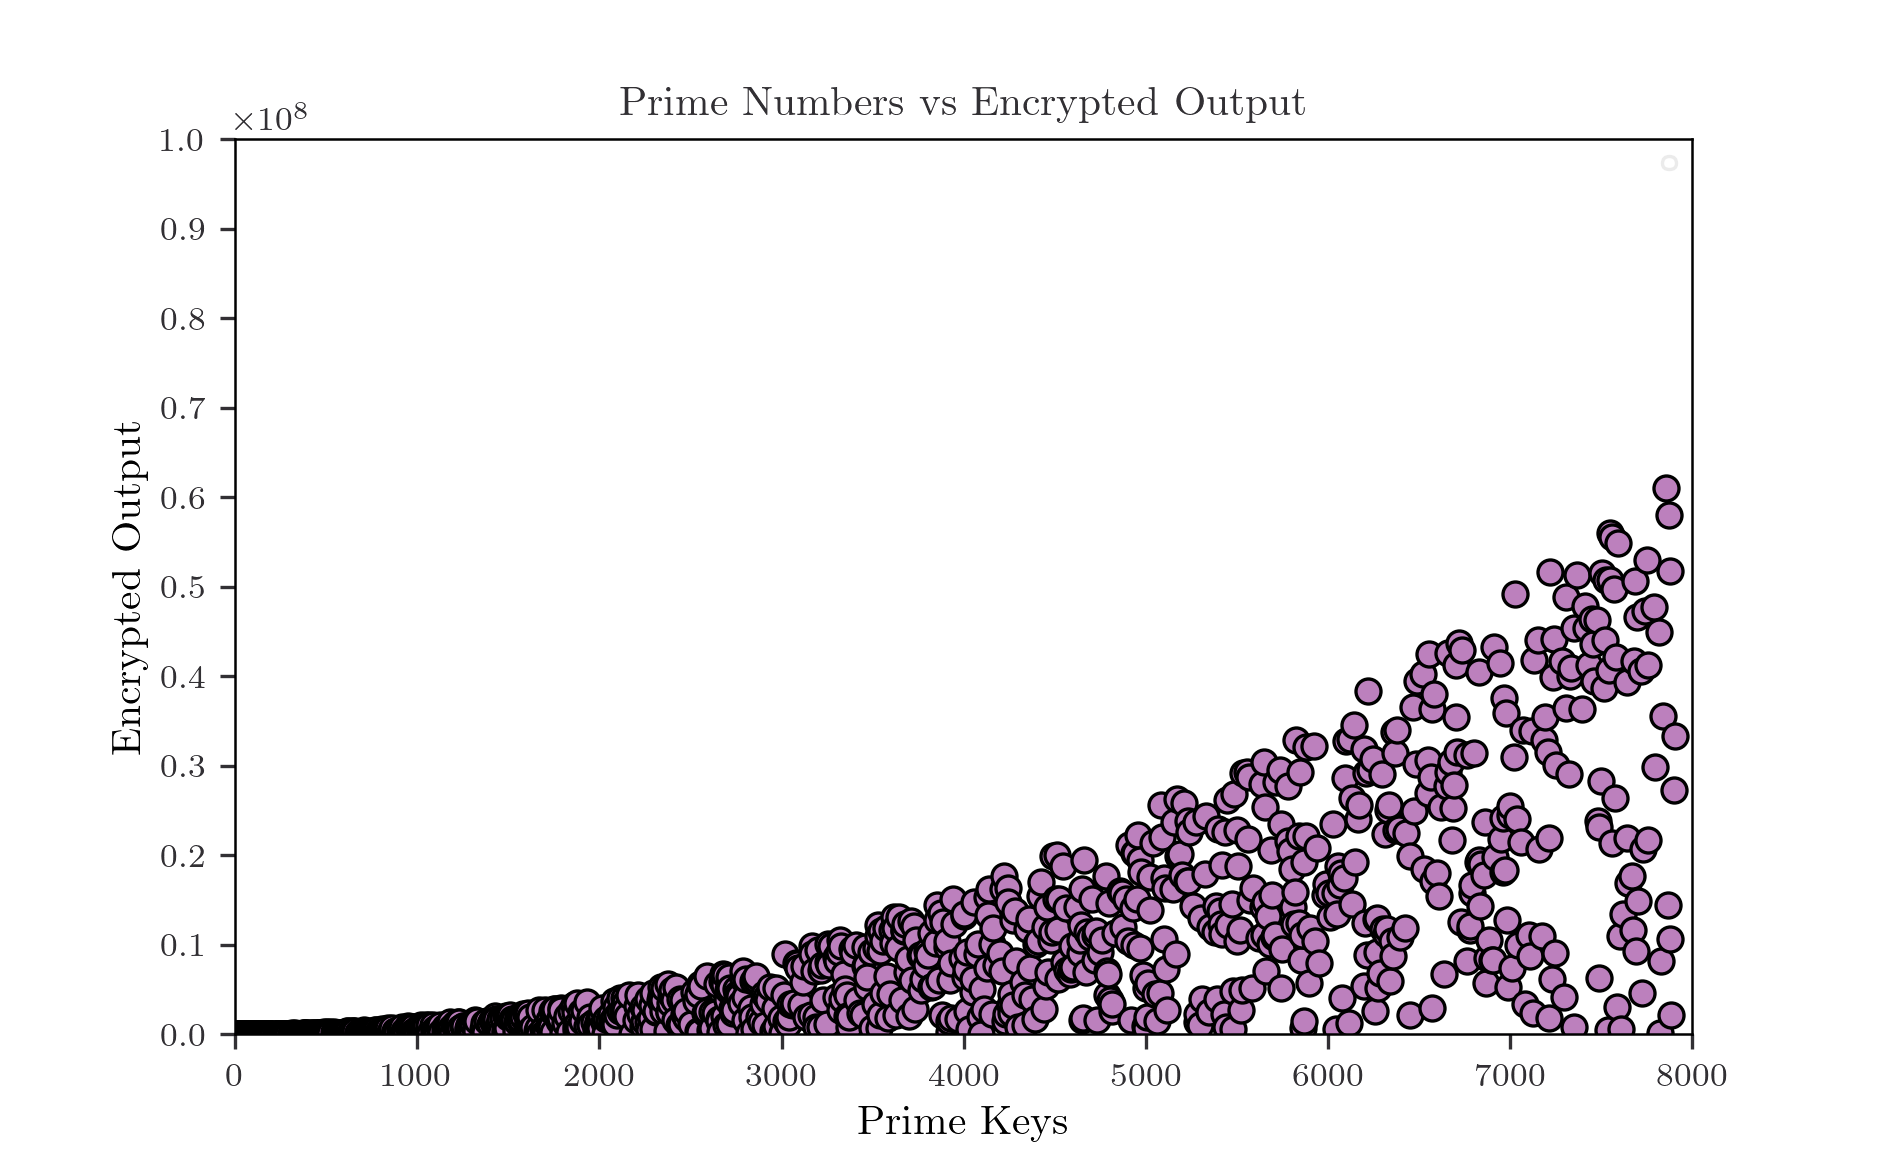
\includegraphics{/comparison/firstterm.png}
\end{figure}

\subsection{Analysis}\label{sec:section6.2}
As seen in the graph above, $p$ and $q$ don't have a direct correlation with the encrypted output since the encrypted message can be any number within a range of values, meaning that it is impossible to determine the prime values used to generate $n$ solely from an encrypted message. That being said, there does appear to be a clear relationship between the primes and encrypted outputs, particularly when it comes to the maximum encrypted output of a message given a range of possible values. The reason why there is a clear maximum value that an encrypted message can have given specific primes is that the encryption process behind RSA uses modulus $n$, specifically 

$$
c \equiv m^{e} \pmod{n}
$$

Whenever you take the modulus of a number, the result is always between 0 and the modulus minus 1. Hence, the maximum value that $c$ can have will always be $n-1$, as $n$ is congruent to $0 \pmod{n}$ and larger numbers will just continue to 'loop' within the modulus $n$. Because of this property, we can plot $P_{n} \cdot P_{n+1} -1$ which represents the maximum possible value for a message that has been encrypted using any pair of prime factors. The graph below highlights possible and impossible encrypted outputs for the first thousand prime pairs.

\begin{figure}[H]
    \centering
    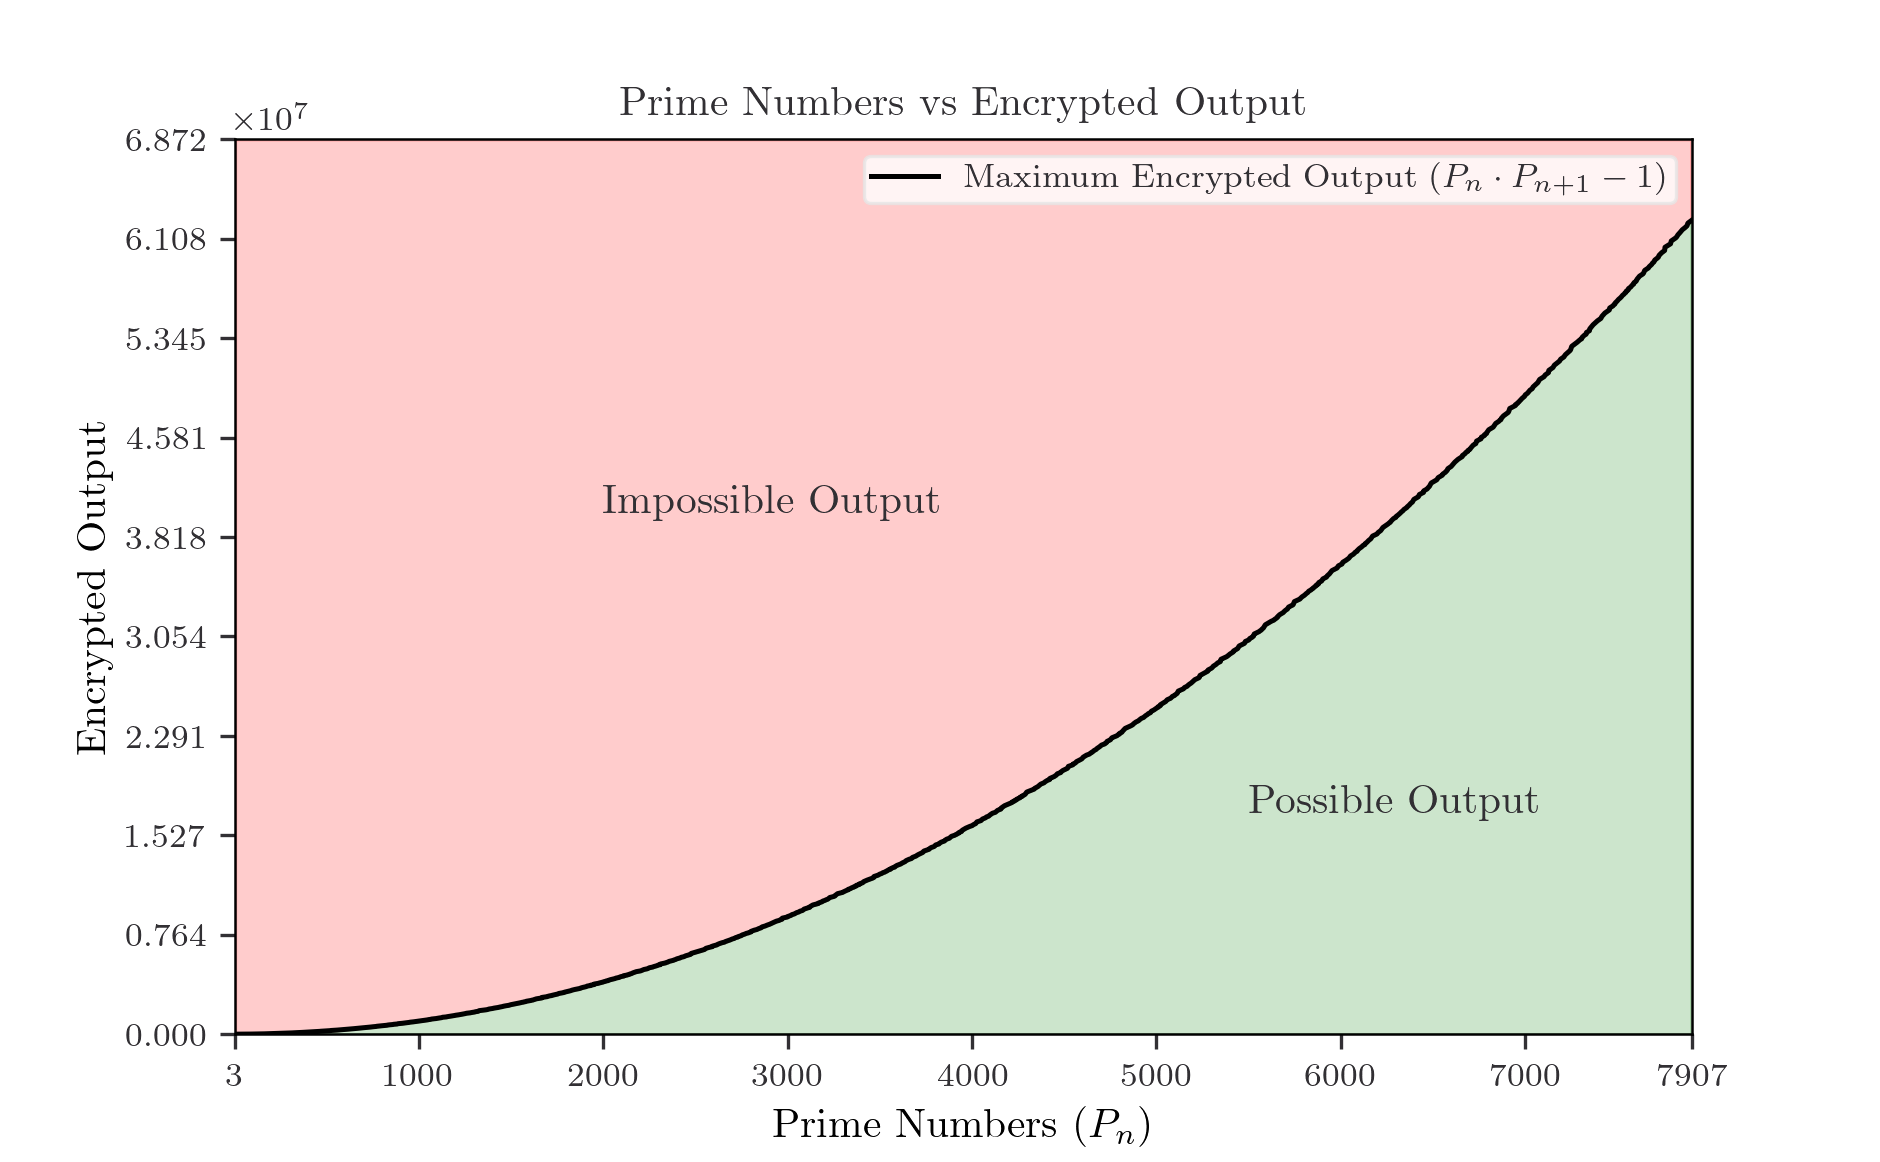
\includegraphics{/comparison/prime_comparison.png}
\end{figure}

The figures above help illustrate how an attacker could exploit mathematical vulnerabilities within RSA in order to determine the private exponent used and decrypt messages.
Firstly, attackers could find $n$ if they used encrypted messages to determine the maximum encrypted output $(n-1)$. While $n$ is part of the public key, it is oftentimes not displayed to users in computer software since the entire RSA encryption and decryption processes happen in the background.
Secondly, using Property (\ref{eq:4}), we know that an attacker could use $n$, more specifically, $\lambda(n)$, to derive $d$ and decrypt messages.

Although both of the aforementioned vulnerabilities that I found in the RSA cryptosystem could be exploited, I concluded that these could be avoided entirely by following a few key generation guidelines. At its core, RSA’s last line of defense relies on its use of prime numbers. While the carmichael function can be used to derive $d$ from $n$, finding it requires one to split $n$ into its two prime factors $(p,q)$. This is straightforward for someone who already knows the values of $p, q$. What about someone who only knows the value of $n$? Assuming that both primes were discarded, and remain unknown, deriving $p$ and $q$ from $n$ could be practically impossible due to prime factorization complexity. Since $n$ is the product of two primes, it has no obvious factors other than $p$ and $q$ themselves. This can make it extremely computationally challenging to factor $n$. Factoring such numbers is done using exhaustive search algorithms; these become increasingly slow as the size of $n$ increases, uncovering two methods to negate the found vulnerabilities.

Firstly, choosing extremely large prime numbers as $p$ and $q$ strengthens the security of RSA, since $n$ will become exponentially larger as $p$ and $q$ grow, creating so many possible encryption values that it would become far too impractical for an attacker to estimate the value of $n$ from encrypted messages. Furthermore, while keeping $n$ hidden would be beneficial in instances where $n$ could be factored, the use of large primes makes this computationally impossible, eliminating the possibility of someone deriving $d$ from $n$.

Secondly, using primes that are significantly different in magnitude makes it too impractical for an attacker to try to find an exact value of $n$. Since larger values result in more primes between $0$ and $n$, testing all permutations of the product of any two primes would be useless when there is no known relationship between $p$ and $q$. In the analysis I conducted, prime factors are always two consecutive primes, meaning they are always a prime number and the next prime number in sequence. I chose to use consecutive primes intentionally, since it clearly demonstrates how the increase in magnitude for both factors contribute to the exponential increase in the range of possible values for $c$. In this instance, it would be obvious that $p$ and $q$ must be of a relatively similar magnitude, since they are consecutive prime numbers. This would enable an attacker to test a significantly smaller range of possible values, since both numbers are known to be consecutive primes near $\sqrt{n}$. In contrast, using primes that are different in magnitude and have been chosen randomly ensures that there is no way to reduce the permutations of $n$ without running the risk of completely skipping the correct pair of prime numbers.
\section{Conclusion}
\label{sec:section7}
This paper studied the behavior of various mathematical concepts within the RSA cryptosystem, and the ways in which they interact with each other to ensure the reliability and security of the encryption process. In addition to this, properties of the cyclic groups that make up RSA were used to uncover possible vulnerabilities, these properties include the relationship between the modulus and the possible encrypted values of a message, as well as the congruence between the public and private exponents within modulo $\lambda (n)$. I placed particular focus on how the observed mathematical relationships could be used to find exploits in the security of the encryption and decryption processes; and the ways in which the same properties can be used to work around these flaws. An interesting approach to further research would be to conduct a similar analysis on other cryptosystems and compare them to RSA.

Overall, this exploration presents meaningful insight that could be beneficial to the security of RSA users, the changes that were proven to strengthen RSA are the use of large prime factors, and the large differences in magnitude between these. 


\pagebreak

\addcontentsline{toc}{section}{References}
\bibliographystyle{apalike}
\bibliography{references}

\end{document}